% Options for packages loaded elsewhere
\PassOptionsToPackage{unicode}{hyperref}
\PassOptionsToPackage{hyphens}{url}
%
\documentclass[
]{article}
\usepackage{amsmath,amssymb}
\usepackage{lmodern}
\usepackage{ifxetex,ifluatex}
\ifnum 0\ifxetex 1\fi\ifluatex 1\fi=0 % if pdftex
  \usepackage[T1]{fontenc}
  \usepackage[utf8]{inputenc}
  \usepackage{textcomp} % provide euro and other symbols
\else % if luatex or xetex
  \usepackage{unicode-math}
  \defaultfontfeatures{Scale=MatchLowercase}
  \defaultfontfeatures[\rmfamily]{Ligatures=TeX,Scale=1}
\fi
% Use upquote if available, for straight quotes in verbatim environments
\IfFileExists{upquote.sty}{\usepackage{upquote}}{}
\IfFileExists{microtype.sty}{% use microtype if available
  \usepackage[]{microtype}
  \UseMicrotypeSet[protrusion]{basicmath} % disable protrusion for tt fonts
}{}
\makeatletter
\@ifundefined{KOMAClassName}{% if non-KOMA class
  \IfFileExists{parskip.sty}{%
    \usepackage{parskip}
  }{% else
    \setlength{\parindent}{0pt}
    \setlength{\parskip}{6pt plus 2pt minus 1pt}}
}{% if KOMA class
  \KOMAoptions{parskip=half}}
\makeatother
\usepackage{xcolor}
\IfFileExists{xurl.sty}{\usepackage{xurl}}{} % add URL line breaks if available
\IfFileExists{bookmark.sty}{\usepackage{bookmark}}{\usepackage{hyperref}}
\hypersetup{
  pdftitle={542\_assign2\_2},
  pdfauthor={Tian Ni},
  hidelinks,
  pdfcreator={LaTeX via pandoc}}
\urlstyle{same} % disable monospaced font for URLs
\usepackage[margin=1in]{geometry}
\usepackage{color}
\usepackage{fancyvrb}
\newcommand{\VerbBar}{|}
\newcommand{\VERB}{\Verb[commandchars=\\\{\}]}
\DefineVerbatimEnvironment{Highlighting}{Verbatim}{commandchars=\\\{\}}
% Add ',fontsize=\small' for more characters per line
\usepackage{framed}
\definecolor{shadecolor}{RGB}{248,248,248}
\newenvironment{Shaded}{\begin{snugshade}}{\end{snugshade}}
\newcommand{\AlertTok}[1]{\textcolor[rgb]{0.94,0.16,0.16}{#1}}
\newcommand{\AnnotationTok}[1]{\textcolor[rgb]{0.56,0.35,0.01}{\textbf{\textit{#1}}}}
\newcommand{\AttributeTok}[1]{\textcolor[rgb]{0.77,0.63,0.00}{#1}}
\newcommand{\BaseNTok}[1]{\textcolor[rgb]{0.00,0.00,0.81}{#1}}
\newcommand{\BuiltInTok}[1]{#1}
\newcommand{\CharTok}[1]{\textcolor[rgb]{0.31,0.60,0.02}{#1}}
\newcommand{\CommentTok}[1]{\textcolor[rgb]{0.56,0.35,0.01}{\textit{#1}}}
\newcommand{\CommentVarTok}[1]{\textcolor[rgb]{0.56,0.35,0.01}{\textbf{\textit{#1}}}}
\newcommand{\ConstantTok}[1]{\textcolor[rgb]{0.00,0.00,0.00}{#1}}
\newcommand{\ControlFlowTok}[1]{\textcolor[rgb]{0.13,0.29,0.53}{\textbf{#1}}}
\newcommand{\DataTypeTok}[1]{\textcolor[rgb]{0.13,0.29,0.53}{#1}}
\newcommand{\DecValTok}[1]{\textcolor[rgb]{0.00,0.00,0.81}{#1}}
\newcommand{\DocumentationTok}[1]{\textcolor[rgb]{0.56,0.35,0.01}{\textbf{\textit{#1}}}}
\newcommand{\ErrorTok}[1]{\textcolor[rgb]{0.64,0.00,0.00}{\textbf{#1}}}
\newcommand{\ExtensionTok}[1]{#1}
\newcommand{\FloatTok}[1]{\textcolor[rgb]{0.00,0.00,0.81}{#1}}
\newcommand{\FunctionTok}[1]{\textcolor[rgb]{0.00,0.00,0.00}{#1}}
\newcommand{\ImportTok}[1]{#1}
\newcommand{\InformationTok}[1]{\textcolor[rgb]{0.56,0.35,0.01}{\textbf{\textit{#1}}}}
\newcommand{\KeywordTok}[1]{\textcolor[rgb]{0.13,0.29,0.53}{\textbf{#1}}}
\newcommand{\NormalTok}[1]{#1}
\newcommand{\OperatorTok}[1]{\textcolor[rgb]{0.81,0.36,0.00}{\textbf{#1}}}
\newcommand{\OtherTok}[1]{\textcolor[rgb]{0.56,0.35,0.01}{#1}}
\newcommand{\PreprocessorTok}[1]{\textcolor[rgb]{0.56,0.35,0.01}{\textit{#1}}}
\newcommand{\RegionMarkerTok}[1]{#1}
\newcommand{\SpecialCharTok}[1]{\textcolor[rgb]{0.00,0.00,0.00}{#1}}
\newcommand{\SpecialStringTok}[1]{\textcolor[rgb]{0.31,0.60,0.02}{#1}}
\newcommand{\StringTok}[1]{\textcolor[rgb]{0.31,0.60,0.02}{#1}}
\newcommand{\VariableTok}[1]{\textcolor[rgb]{0.00,0.00,0.00}{#1}}
\newcommand{\VerbatimStringTok}[1]{\textcolor[rgb]{0.31,0.60,0.02}{#1}}
\newcommand{\WarningTok}[1]{\textcolor[rgb]{0.56,0.35,0.01}{\textbf{\textit{#1}}}}
\usepackage{graphicx}
\makeatletter
\def\maxwidth{\ifdim\Gin@nat@width>\linewidth\linewidth\else\Gin@nat@width\fi}
\def\maxheight{\ifdim\Gin@nat@height>\textheight\textheight\else\Gin@nat@height\fi}
\makeatother
% Scale images if necessary, so that they will not overflow the page
% margins by default, and it is still possible to overwrite the defaults
% using explicit options in \includegraphics[width, height, ...]{}
\setkeys{Gin}{width=\maxwidth,height=\maxheight,keepaspectratio}
% Set default figure placement to htbp
\makeatletter
\def\fps@figure{htbp}
\makeatother
\setlength{\emergencystretch}{3em} % prevent overfull lines
\providecommand{\tightlist}{%
  \setlength{\itemsep}{0pt}\setlength{\parskip}{0pt}}
\setcounter{secnumdepth}{-\maxdimen} % remove section numbering
\ifluatex
  \usepackage{selnolig}  % disable illegal ligatures
\fi

\title{542\_assign2\_2}
\author{Tian Ni}
\date{9/23/2021}

\begin{document}
\maketitle

\begin{Shaded}
\begin{Highlighting}[]
\FunctionTok{library}\NormalTok{(glmnet)}
\end{Highlighting}
\end{Shaded}

\begin{verbatim}
## 载入需要的程辑包:Matrix
\end{verbatim}

\begin{verbatim}
## Loaded glmnet 4.1-2
\end{verbatim}

\begin{Shaded}
\begin{Highlighting}[]
\FunctionTok{library}\NormalTok{(pls)}
\end{Highlighting}
\end{Shaded}

\begin{verbatim}
## 
## 载入程辑包:'pls'
\end{verbatim}

\begin{verbatim}
## The following object is masked from 'package:stats':
## 
##     loadings
\end{verbatim}

\begin{Shaded}
\begin{Highlighting}[]
\FunctionTok{set.seed}\NormalTok{(}\DecValTok{6659}\NormalTok{)}
\end{Highlighting}
\end{Shaded}

Load the data

\begin{Shaded}
\begin{Highlighting}[]
\NormalTok{myData}\OtherTok{=}\FunctionTok{read.csv}\NormalTok{(}\StringTok{"BostonData2.csv"}\NormalTok{)}
\NormalTok{myData}\OtherTok{=}\NormalTok{myData[,}\SpecialCharTok{{-}}\DecValTok{1}\NormalTok{]}
\FunctionTok{dim}\NormalTok{(myData)}
\end{Highlighting}
\end{Shaded}

\begin{verbatim}
## [1] 506  92
\end{verbatim}

\begin{Shaded}
\begin{Highlighting}[]
\NormalTok{X}\OtherTok{=}\FunctionTok{data.matrix}\NormalTok{(myData[,}\SpecialCharTok{{-}}\DecValTok{1}\NormalTok{])}
\NormalTok{Y}\OtherTok{=}\FunctionTok{data.matrix}\NormalTok{(myData[,}\DecValTok{1}\NormalTok{])}
\end{Highlighting}
\end{Shaded}

Then we construct those seven procedure to make it easier to read

\begin{Shaded}
\begin{Highlighting}[]
\NormalTok{T}\OtherTok{=}\DecValTok{50}
\NormalTok{n}\OtherTok{=}\FunctionTok{length}\NormalTok{(Y)}
\NormalTok{ntest}\OtherTok{=}\FunctionTok{round}\NormalTok{(n}\SpecialCharTok{*}\FloatTok{0.25}\NormalTok{)}
\NormalTok{sample}\OtherTok{=}\FunctionTok{sample}\NormalTok{(n,ntest)}
\NormalTok{test}\OtherTok{=}\NormalTok{myData[sample,]}
\NormalTok{train}\OtherTok{=}\NormalTok{myData[}\SpecialCharTok{{-}}\NormalTok{sample,]}
\end{Highlighting}
\end{Shaded}

\begin{Shaded}
\begin{Highlighting}[]
\NormalTok{full}\OtherTok{=}\ControlFlowTok{function}\NormalTok{(train,test)\{}
\NormalTok{  full.model}\OtherTok{=}\FunctionTok{lm}\NormalTok{(Y}\SpecialCharTok{\textasciitilde{}}\NormalTok{.,}\AttributeTok{data =}\NormalTok{ train)}
\NormalTok{  y.pred}\OtherTok{=}\FunctionTok{predict}\NormalTok{(full.model,}\AttributeTok{newdata=}\NormalTok{test)}
\NormalTok{  MSPE}\OtherTok{=}\FunctionTok{mean}\NormalTok{((test}\SpecialCharTok{$}\NormalTok{Y}\SpecialCharTok{{-}}\NormalTok{y.pred)}\SpecialCharTok{\^{}}\DecValTok{2}\NormalTok{)}
  \FunctionTok{return}\NormalTok{(MSPE)}
\NormalTok{\}}
\end{Highlighting}
\end{Shaded}

\begin{Shaded}
\begin{Highlighting}[]
\DocumentationTok{\#\# For ridge regression, we need first find the correct range of lambda}
\NormalTok{cv.out}\OtherTok{=}\FunctionTok{cv.glmnet}\NormalTok{(X[}\SpecialCharTok{{-}}\NormalTok{sample,],Y[}\SpecialCharTok{{-}}\NormalTok{sample],}\AttributeTok{alpha=}\DecValTok{0}\NormalTok{)}
\NormalTok{best.lam}\OtherTok{=}\NormalTok{cv.out}\SpecialCharTok{$}\NormalTok{lambda.min}
\FunctionTok{sum}\NormalTok{(cv.out}\SpecialCharTok{$}\NormalTok{lambda}\SpecialCharTok{\textless{}}\NormalTok{best.lam)}
\end{Highlighting}
\end{Shaded}

\begin{verbatim}
## [1] 0
\end{verbatim}

\begin{Shaded}
\begin{Highlighting}[]
\FunctionTok{plot}\NormalTok{(cv.out)}
\end{Highlighting}
\end{Shaded}

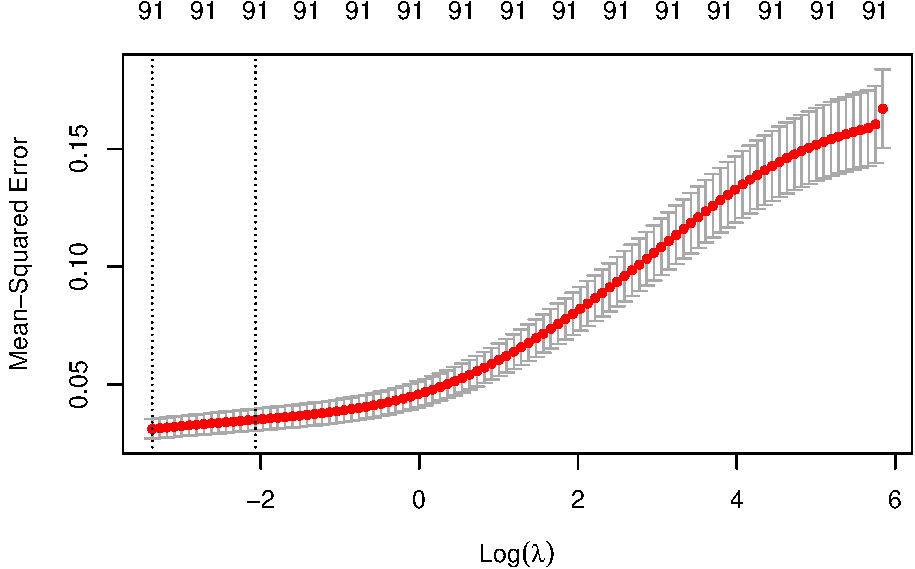
\includegraphics{542_assign2_2_files/figure-latex/unnamed-chunk-5-1.pdf}

\begin{Shaded}
\begin{Highlighting}[]
\CommentTok{\# Try a lower lambda range to get the lowest MSPE}
\NormalTok{mylasso.lambda.seq}\OtherTok{=}\FunctionTok{exp}\NormalTok{(}\FunctionTok{seq}\NormalTok{(}\SpecialCharTok{{-}}\DecValTok{10}\NormalTok{,}\SpecialCharTok{{-}}\DecValTok{2}\NormalTok{,}\AttributeTok{length.out=}\DecValTok{100}\NormalTok{))}
\NormalTok{cv.out}\OtherTok{=}\FunctionTok{cv.glmnet}\NormalTok{(X[}\SpecialCharTok{{-}}\NormalTok{sample,],Y[}\SpecialCharTok{{-}}\NormalTok{sample],}\AttributeTok{alpha=}\DecValTok{0}\NormalTok{,}\AttributeTok{lambda =}\NormalTok{ mylasso.lambda.seq) }
\FunctionTok{plot}\NormalTok{(cv.out)   }
\end{Highlighting}
\end{Shaded}

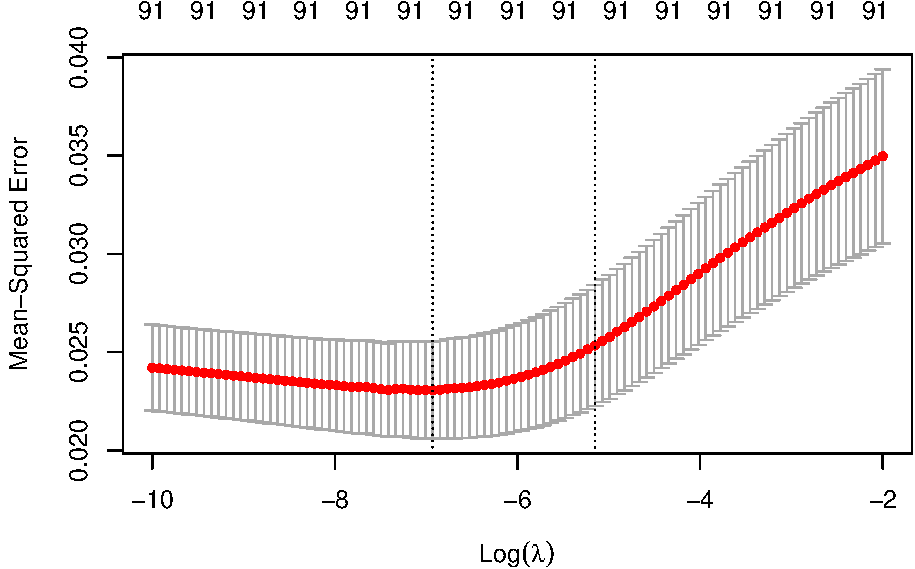
\includegraphics{542_assign2_2_files/figure-latex/unnamed-chunk-5-2.pdf}

Now we found the range of lambda, construct the ridge function

\begin{Shaded}
\begin{Highlighting}[]
\NormalTok{ridge}\OtherTok{=}\ControlFlowTok{function}\NormalTok{(xtrain,xtest,ytrain,ytest)\{}
\NormalTok{  cv.out}\OtherTok{=}\FunctionTok{cv.glmnet}\NormalTok{(xtrain,ytrain,}\AttributeTok{alpha=}\DecValTok{0}\NormalTok{,}\AttributeTok{lambda =}\NormalTok{ mylasso.lambda.seq) }
\NormalTok{  best.lam}\OtherTok{=}\NormalTok{cv.out}\SpecialCharTok{$}\NormalTok{lambda.min}
\NormalTok{  Ytest.pred}\OtherTok{=}\FunctionTok{predict}\NormalTok{(cv.out,}\AttributeTok{s=}\NormalTok{best.lam,}\AttributeTok{newx=}\NormalTok{xtest)}
\NormalTok{  ridge.min}\OtherTok{=}\FunctionTok{mean}\NormalTok{((ytest}\SpecialCharTok{{-}}\NormalTok{Ytest.pred)}\SpecialCharTok{\^{}}\DecValTok{2}\NormalTok{)}
\NormalTok{  best.lam}\OtherTok{=}\NormalTok{cv.out}\SpecialCharTok{$}\NormalTok{lambda}\FloatTok{.1}\NormalTok{se}
\NormalTok{  Ytest.pred}\OtherTok{=}\FunctionTok{predict}\NormalTok{(cv.out,}\AttributeTok{s=}\NormalTok{best.lam,}\AttributeTok{newx=}\NormalTok{xtest)}
\NormalTok{  ridge}\FloatTok{.1}\NormalTok{se}\OtherTok{=}\FunctionTok{mean}\NormalTok{((ytest}\SpecialCharTok{{-}}\NormalTok{Ytest.pred)}\SpecialCharTok{\^{}}\DecValTok{2}\NormalTok{)}
  
  \FunctionTok{return}\NormalTok{(}\FunctionTok{c}\NormalTok{(ridge.min,ridge}\FloatTok{.1}\NormalTok{se))}
\NormalTok{\}}

\FunctionTok{ridge}\NormalTok{(X[}\SpecialCharTok{{-}}\NormalTok{sample,],X[sample,],Y[}\SpecialCharTok{{-}}\NormalTok{sample,],Y[sample,])[}\DecValTok{1}\NormalTok{]}
\end{Highlighting}
\end{Shaded}

\begin{verbatim}
## [1] 0.02872024
\end{verbatim}

Now we look at the lasso function

\begin{Shaded}
\begin{Highlighting}[]
\NormalTok{lasso}\OtherTok{=}\ControlFlowTok{function}\NormalTok{(xtrain,xtest,ytrain,ytest)\{}
\NormalTok{  cv.out}\OtherTok{=}\FunctionTok{cv.glmnet}\NormalTok{(xtrain,ytrain,}\AttributeTok{alpha=}\DecValTok{1}\NormalTok{)}
\NormalTok{  best.lam}\OtherTok{=}\NormalTok{cv.out}\SpecialCharTok{$}\NormalTok{lambda.min}
\NormalTok{  Ytest.pred}\OtherTok{=}\FunctionTok{predict}\NormalTok{(cv.out,}\AttributeTok{s=}\NormalTok{best.lam,}\AttributeTok{newx=}\NormalTok{xtest)}
\NormalTok{  lasso.min}\OtherTok{=}\FunctionTok{mean}\NormalTok{((ytest}\SpecialCharTok{{-}}\NormalTok{Ytest.pred)}\SpecialCharTok{\^{}}\DecValTok{2}\NormalTok{)}
  
\NormalTok{  best.lam}\OtherTok{=}\NormalTok{cv.out}\SpecialCharTok{$}\NormalTok{lambda}\FloatTok{.1}\NormalTok{se}
\NormalTok{  Ytest.pred}\OtherTok{=}\FunctionTok{predict}\NormalTok{(cv.out,}\AttributeTok{s=}\NormalTok{best.lam,}\AttributeTok{newx=}\NormalTok{xtest)}
\NormalTok{  lasso}\FloatTok{.1}\NormalTok{se}\OtherTok{=}\FunctionTok{mean}\NormalTok{((ytest}\SpecialCharTok{{-}}\NormalTok{Ytest.pred)}\SpecialCharTok{\^{}}\DecValTok{2}\NormalTok{)}
  
\NormalTok{  mylasso.coef}\OtherTok{=}\FunctionTok{predict}\NormalTok{(cv.out,}\AttributeTok{s=}\NormalTok{best.lam,}\AttributeTok{type=}\StringTok{"coefficients"}\NormalTok{)}
\NormalTok{  var.sel}\OtherTok{=}\FunctionTok{row.names}\NormalTok{(mylasso.coef)[}\FunctionTok{which}\NormalTok{(mylasso.coef }\SpecialCharTok{!=} \DecValTok{0}\NormalTok{)[}\SpecialCharTok{{-}}\DecValTok{1}\NormalTok{]]}
\NormalTok{  mylasso.refit}\OtherTok{=}\FunctionTok{lm}\NormalTok{(Y}\SpecialCharTok{\textasciitilde{}}\NormalTok{.,myData[}\SpecialCharTok{{-}}\NormalTok{sample,}\FunctionTok{c}\NormalTok{(}\StringTok{"Y"}\NormalTok{,var.sel)])}
\NormalTok{  Ytest.pred}\OtherTok{=}\FunctionTok{predict}\NormalTok{(mylasso.refit,}\AttributeTok{newdata=}\NormalTok{myData[sample,])}
\NormalTok{  lasso.refit}\OtherTok{=}\FunctionTok{mean}\NormalTok{((Ytest.pred}\SpecialCharTok{{-}}\NormalTok{ytest)}\SpecialCharTok{\^{}}\DecValTok{2}\NormalTok{)}
  
  \FunctionTok{return}\NormalTok{(}\FunctionTok{c}\NormalTok{(lasso.min,lasso}\FloatTok{.1}\NormalTok{se,lasso.refit))}
\NormalTok{\}}

\FunctionTok{lasso}\NormalTok{(X[}\SpecialCharTok{{-}}\NormalTok{sample,],X[sample,],Y[}\SpecialCharTok{{-}}\NormalTok{sample,],Y[sample,])}
\end{Highlighting}
\end{Shaded}

\begin{verbatim}
## [1] 0.02897240 0.03150113 0.03015074
\end{verbatim}

Now we work on the PCR function

\begin{Shaded}
\begin{Highlighting}[]
\NormalTok{myPCR}\OtherTok{=}\ControlFlowTok{function}\NormalTok{(train,ytrain,test,ytest)\{}
\NormalTok{  mypcr}\OtherTok{=}\FunctionTok{pcr}\NormalTok{(Y}\SpecialCharTok{\textasciitilde{}}\NormalTok{., }\AttributeTok{data=}\NormalTok{train,}\AttributeTok{validation=}\StringTok{"CV"}\NormalTok{)}
\NormalTok{  CVerr}\OtherTok{=}\FunctionTok{RMSEP}\NormalTok{(mypcr)}\SpecialCharTok{$}\NormalTok{val[}\DecValTok{1}\NormalTok{, ,]}
\NormalTok{  adjCVerr}\OtherTok{=}\FunctionTok{RMSEP}\NormalTok{(mypcr)}\SpecialCharTok{$}\NormalTok{val[}\DecValTok{2}\NormalTok{, ,]}
\NormalTok{  best.ncomp}\OtherTok{=}\FunctionTok{which.min}\NormalTok{(CVerr)}\SpecialCharTok{{-}}\DecValTok{1}
  \ControlFlowTok{if}\NormalTok{(best.ncomp}\SpecialCharTok{==}\DecValTok{0}\NormalTok{)\{}
\NormalTok{    Ytest.pred}\OtherTok{=}\FunctionTok{mean}\NormalTok{(myData}\SpecialCharTok{$}\NormalTok{Y[}\SpecialCharTok{{-}}\NormalTok{sample])}
\NormalTok{  \}}
  \ControlFlowTok{else}\NormalTok{\{}
\NormalTok{    Ytest.pred}\OtherTok{=}\FunctionTok{predict}\NormalTok{(mypcr,test,}\AttributeTok{ncomp=}\NormalTok{best.ncomp)}
\NormalTok{  \}}
\NormalTok{  pcr}\OtherTok{=}\FunctionTok{mean}\NormalTok{((Ytest.pred}\SpecialCharTok{{-}}\NormalTok{ytest)}\SpecialCharTok{\^{}}\DecValTok{2}\NormalTok{)}
  \FunctionTok{return}\NormalTok{(pcr)}
\NormalTok{\}}
\FunctionTok{myPCR}\NormalTok{(train,train}\SpecialCharTok{$}\NormalTok{Y,test,test}\SpecialCharTok{$}\NormalTok{Y)}
\end{Highlighting}
\end{Shaded}

\begin{verbatim}
## [1] 0.02572769
\end{verbatim}

Run the simulation 50 times

\begin{Shaded}
\begin{Highlighting}[]
\NormalTok{sample}\OtherTok{=}\FunctionTok{sample}\NormalTok{(n,ntest)}
\NormalTok{test}\OtherTok{=}\NormalTok{myData[sample,]}
\NormalTok{train}\OtherTok{=}\NormalTok{myData[}\SpecialCharTok{{-}}\NormalTok{sample,]}
\end{Highlighting}
\end{Shaded}


\end{document}
